% !TEX root = ../../main.tex

\subsection{Thermogravimetry results}

A typical \gls{TGA} curve, as measured on a pristine material
is characterised by three main mass losses: a loss
at low temperature, usually until \SI{100}{\degreeCelsius},
which is indicative of adsorbed water from the environment;
a secondary mass loss in the \SIrange{100}{200}{\degreeCelsius}
range, corresponding to the evacuation of residual solvent 
from the pores and finally, a large step which is a sign of 
sample degradation as the linker is oxidized.

A selection of \gls{TGA} curves measured on the leached samples
can be seen in \autoref{def:fig:tga-dataset}. The complete set of data
can be found in \autoref{appx:def}, \autoref{appx:def:tga}.

\begin{figure}[htbp]
    \centering

    \begin{subfigure}{0.5\linewidth}
        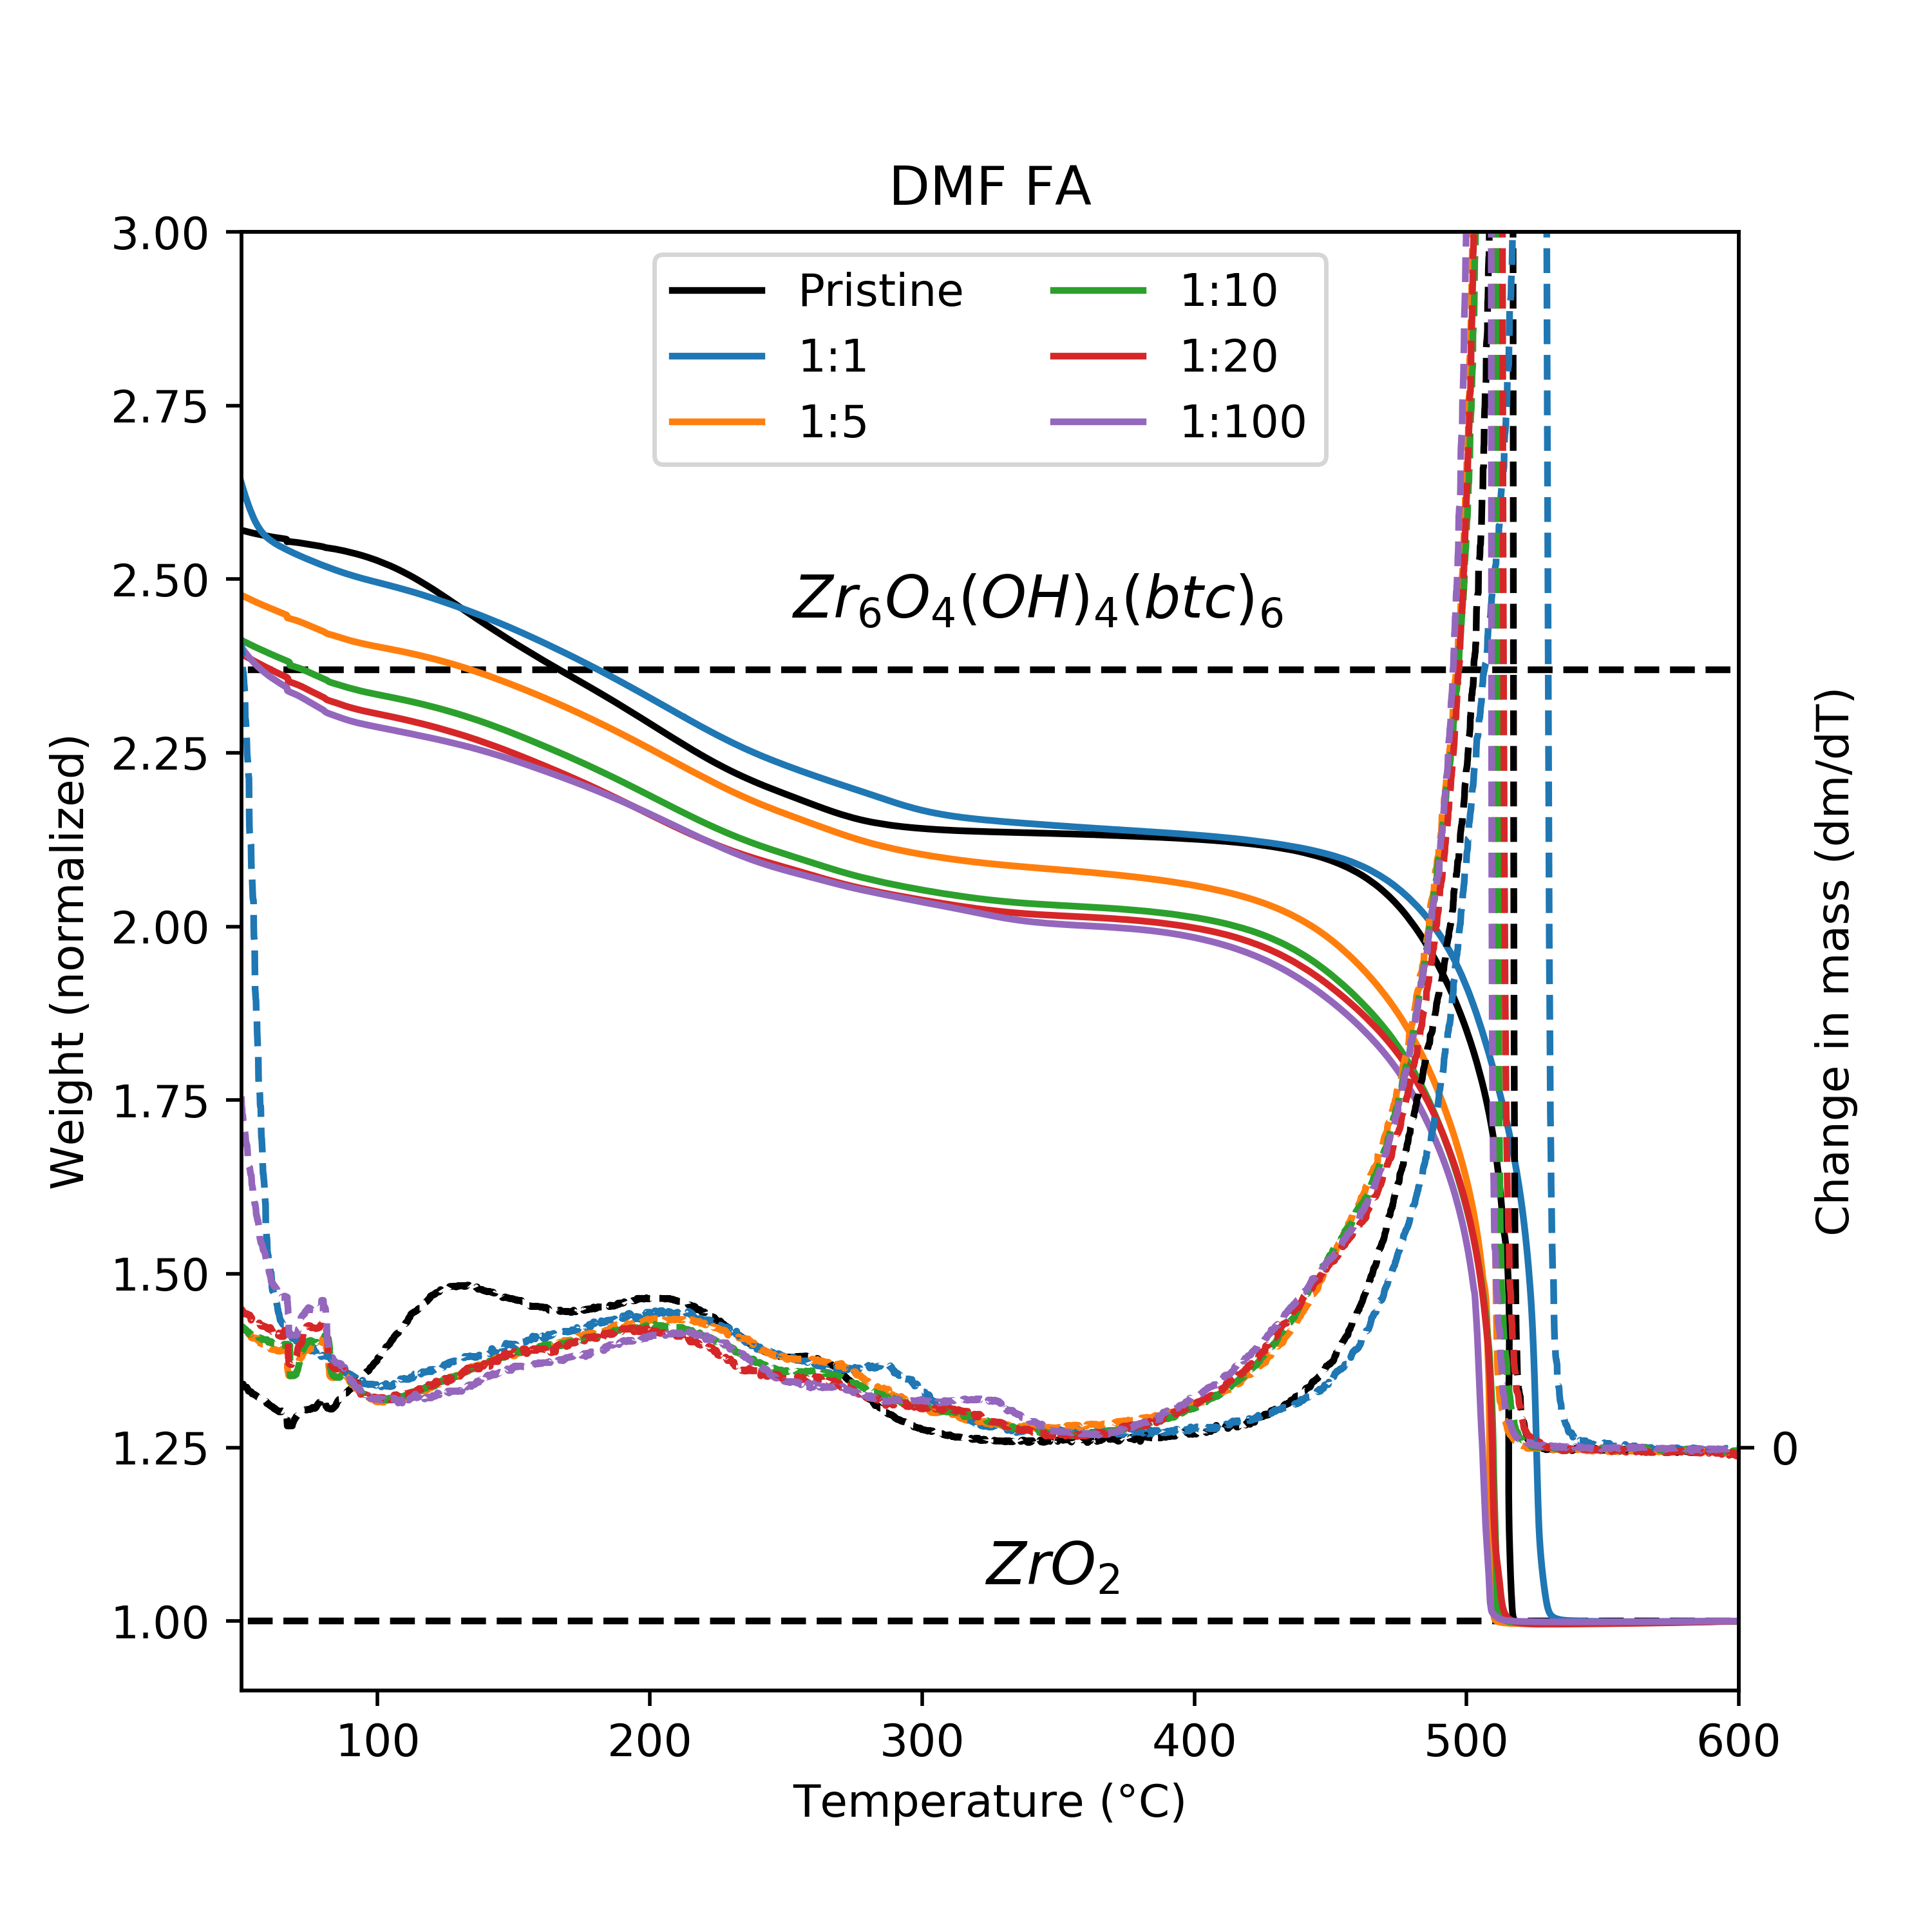
\includegraphics[width=\textwidth]{tga/DMF-FA}%
		\caption{}%
        \label{def:fig:tga-dmf-fa}
    \end{subfigure}%
    \begin{subfigure}{0.5\linewidth}
        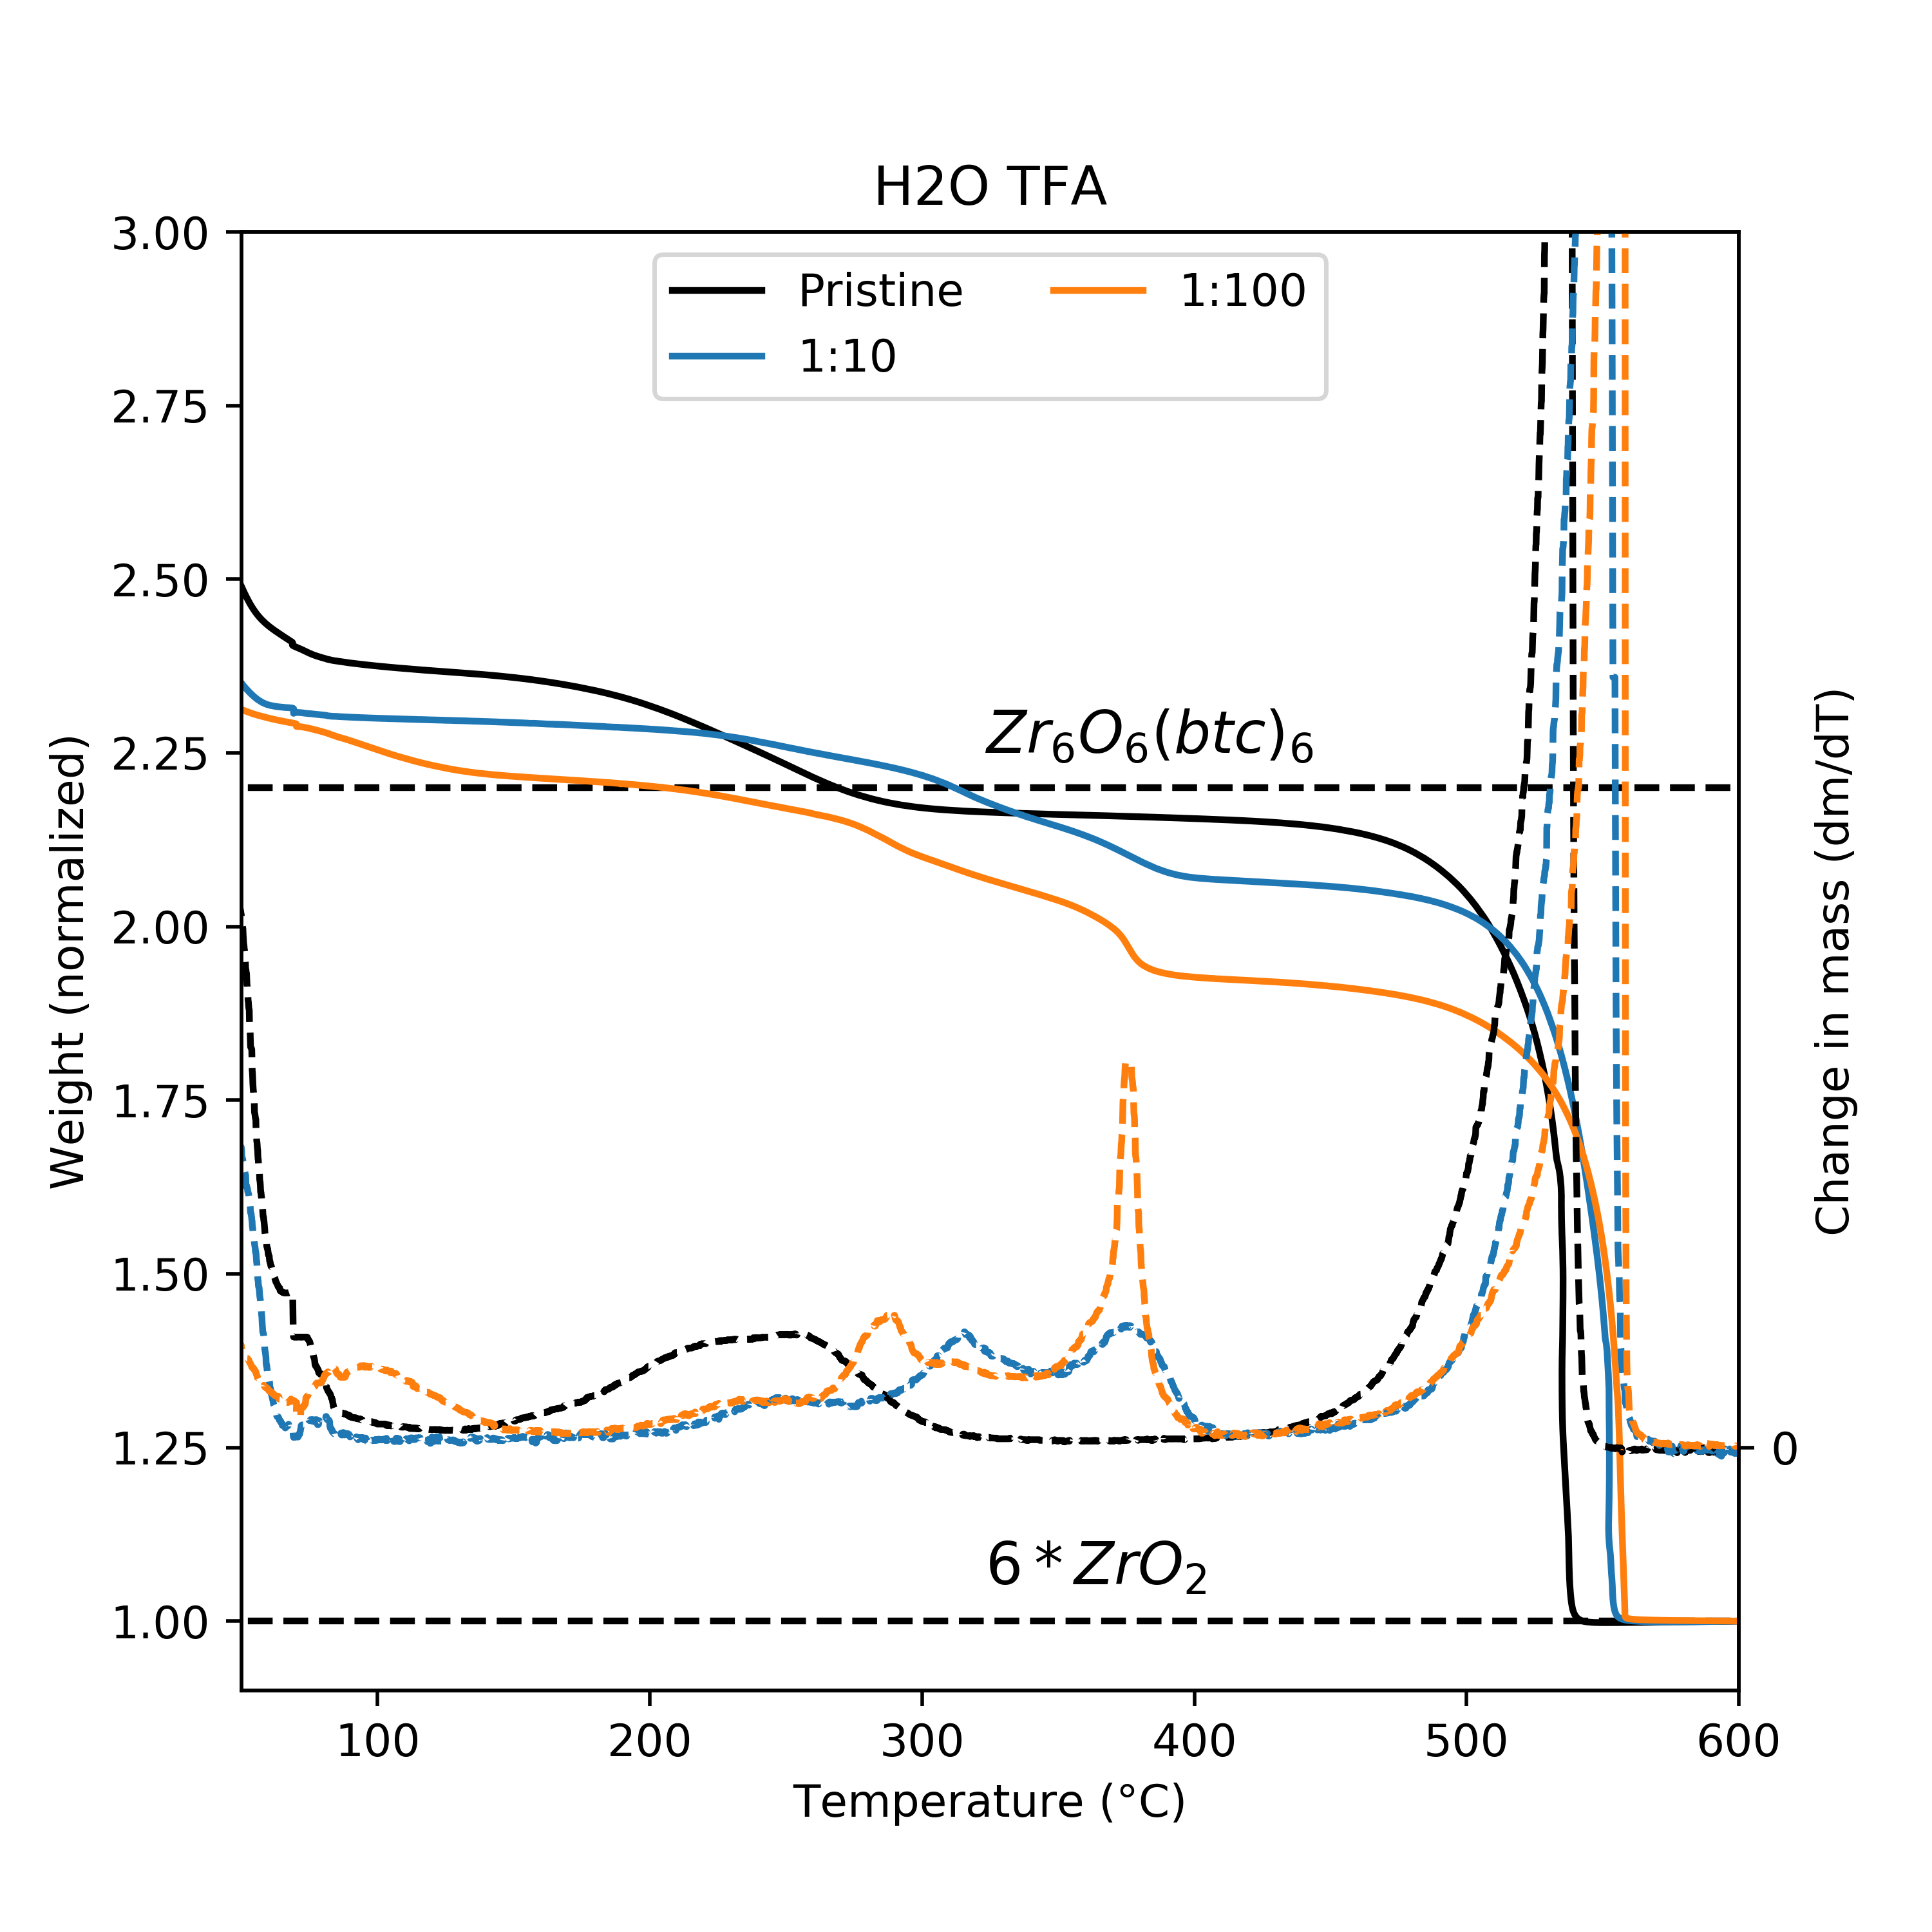
\includegraphics[width=\textwidth]{tga/H2O-TFA}%
		\caption{}%
        \label{def:fig:tga-h2o-tfa}
    \end{subfigure}%

    
    \begin{subfigure}{0.5\linewidth}
        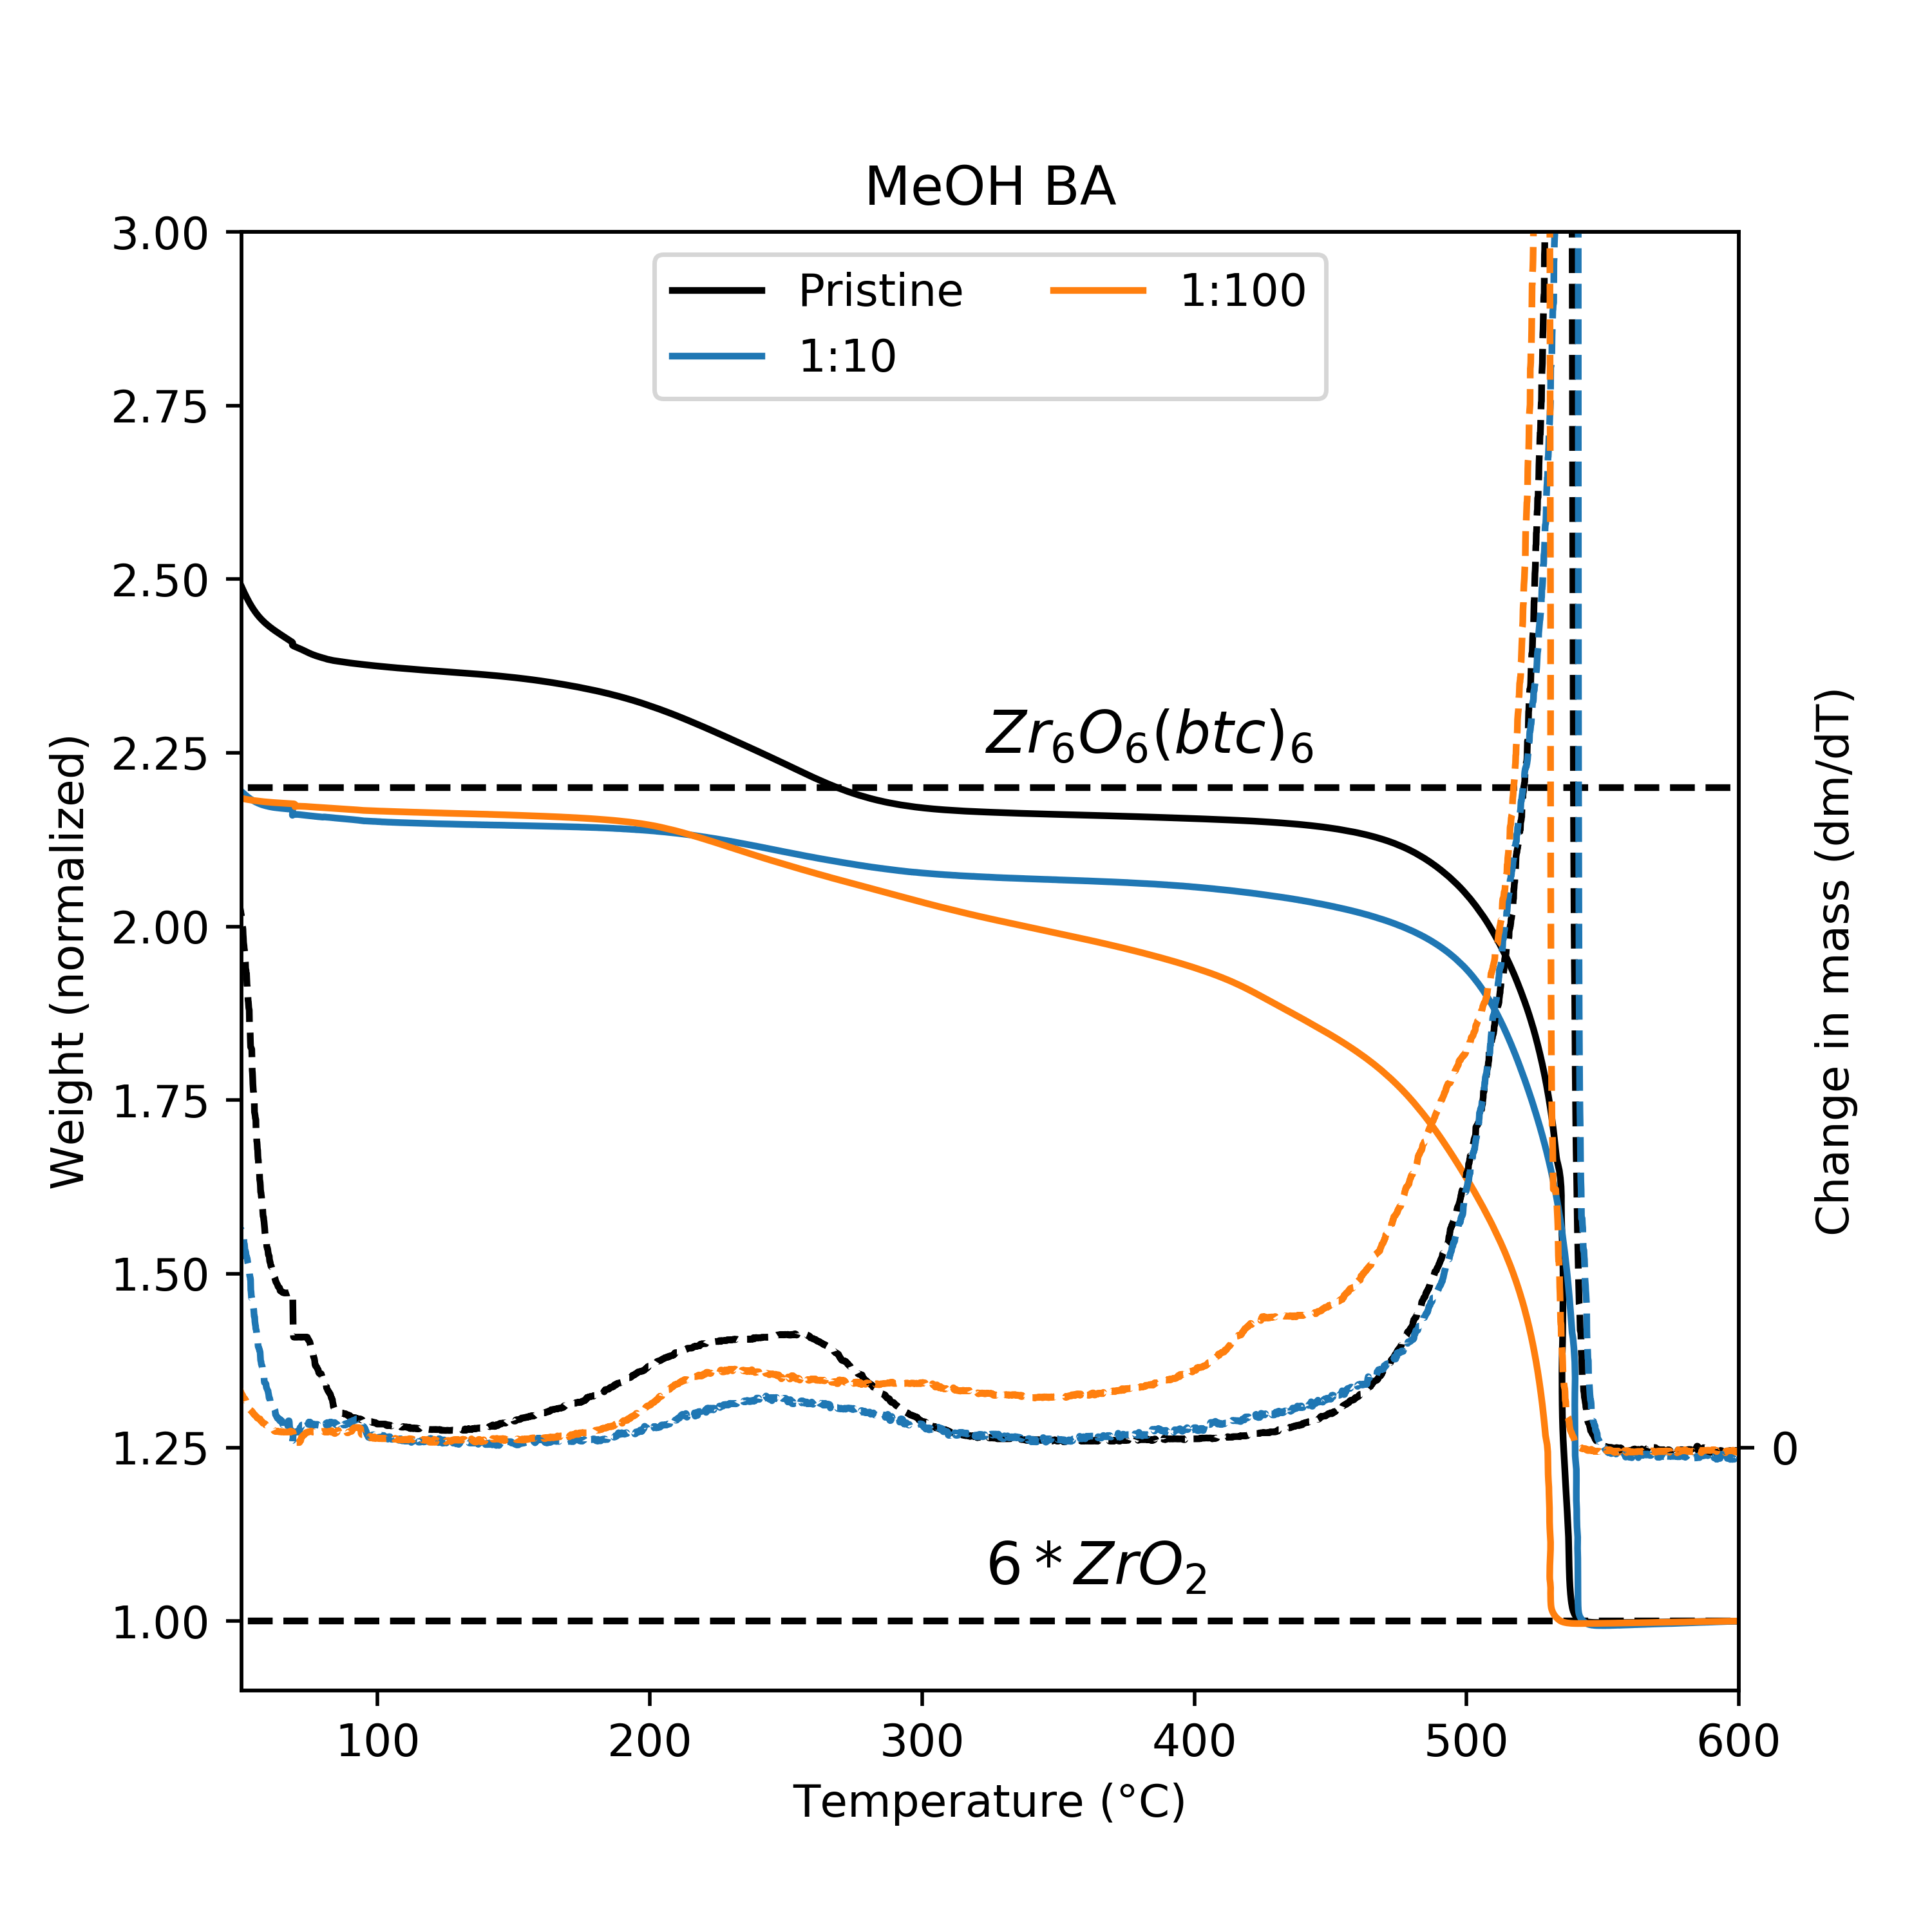
\includegraphics[width=\textwidth]{tga/MeOH-BA}%
		\caption{}%
        \label{def:fig:tga-meoh-ba}
    \end{subfigure}%
    \begin{subfigure}{0.5\linewidth}
        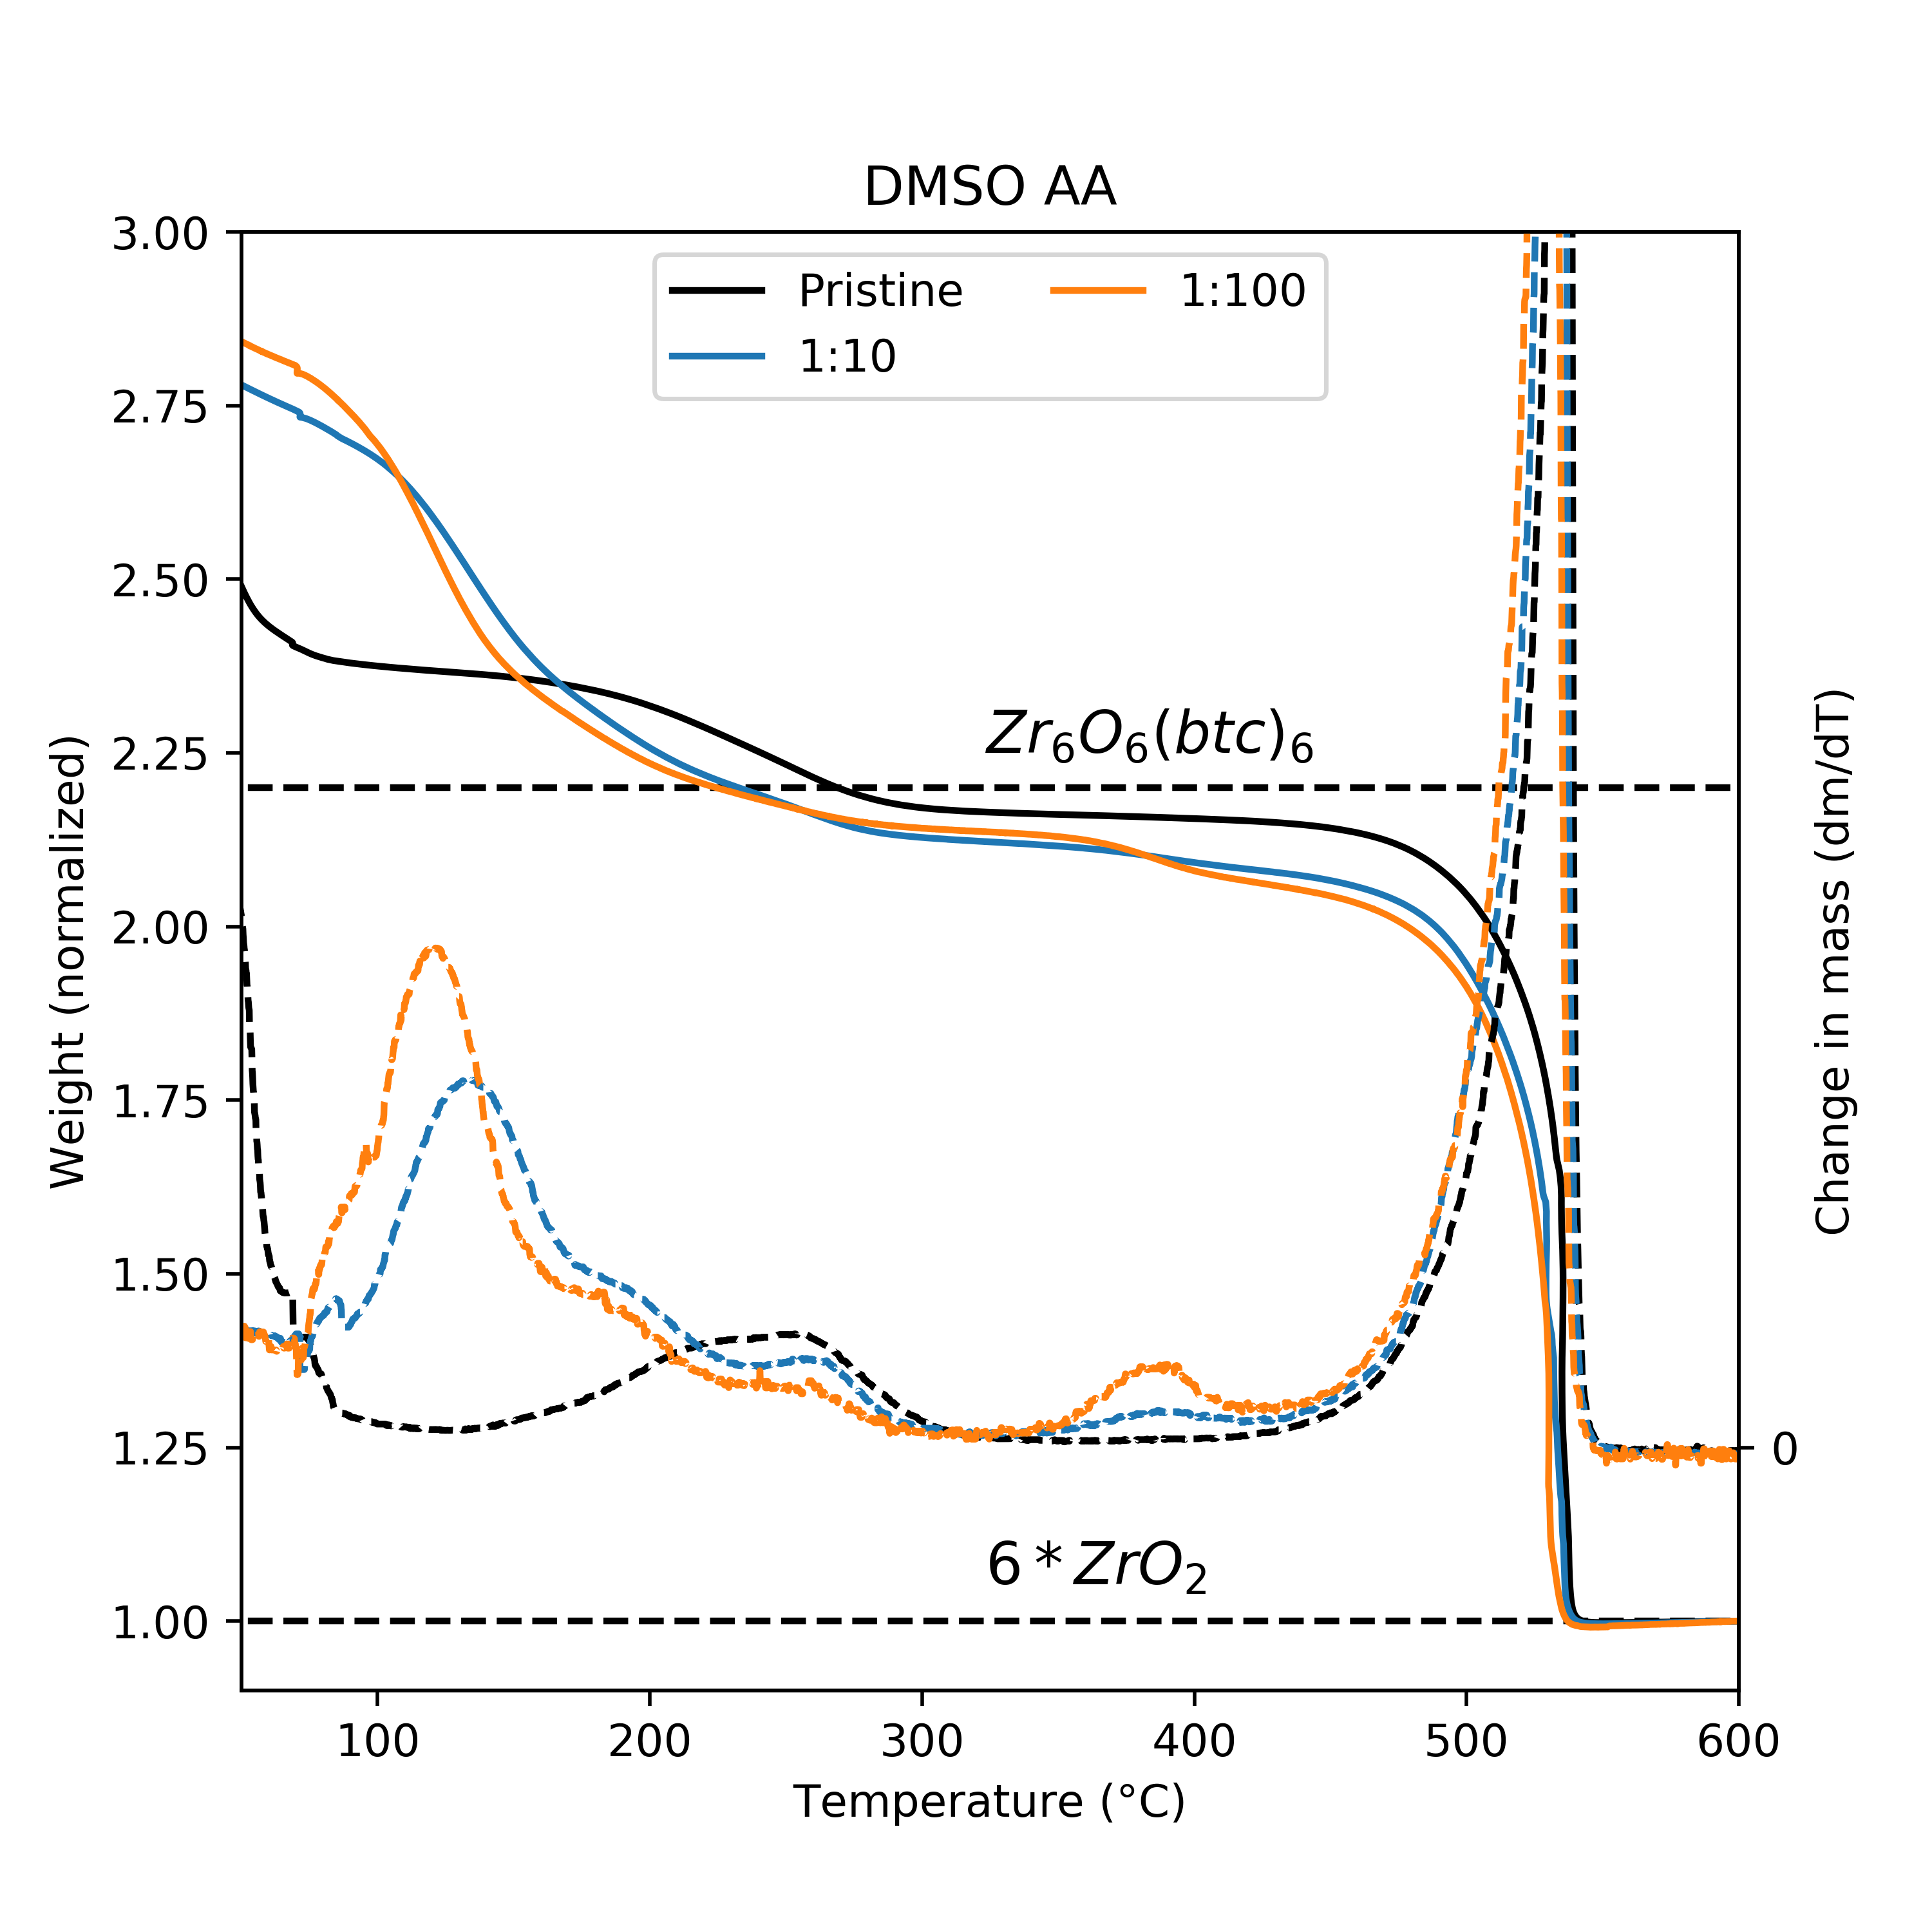
\includegraphics[width=\textwidth]{tga/DMSO-AA}%
		\caption{}%
        \label{def:fig:tga-dmso-aa}
    \end{subfigure}%

    \caption{A selection of the \gls{TGA} curves as measured on the
    leached samples: (a) formic acid in \gls{DMF}, (b) trifluoroacetic
    acid in water, (c) benzoic acid in methanol and (d) acetic acid
    in \gls{DMSO}. The curve for the parent material is in black. 
    Dotted lines correspond to the secondary y axis as a 
    semilogarithm of the first derivative of mass loss with 
    respect to temperature.}%
    \label{def:fig:tga-dataset}
\end{figure}

There are four types of differences that can be arise 
between curves on different samples:

\begin{itemize}
    \item the aforementioned change in overall height,
    which indicates the presence of missing linker defects;
    \item differences in the solvent removal step, as they
    have different boiling points and interactions with the 
    framework;
    \item in case the defects are capped by an agent such as 
    the modulator molecule used, it may introduce a new 
    mass loss step between solvent removal and complete
    structure breakdown;
    \item finally, a highly defective structure loses part 
    of its thermal resistance altering both the onset of mass
    loss and the final decomposition temperature.
\end{itemize}

From the \gls{TGA} curve of the pristine UiO-66 material, 
it is immediately obvious that there are some defects 
already present in the sample. By using the normalized
mass at \SI{420}{\degreeCelsius} a linker-to-cluster 
ratio of around 11.6:1 can be calculated. This shows that
there are still intrinsic defects in the as-synthesised 
structure. These defects are most likely capped by 
formate moieties, which have been generated during 
the solvothermal synthesis in \gls{DMF} through solvent 
self-hydrolysis (\autoref{def:eqn:dmf-hydrolysis}), as 
commercially available solvent has a small percentage of 
residual water~\cite{shearerDefectEngineeringTuning2016}.
%
\begin{equation}\label{def:eqn:dmf-hydrolysis}
    \ce{HCON(CH3)2 + H2O -> HCOOH + HN(CH3)2}
\end{equation}
%
It follows that the mass loss step around \SI{250}{\degreeCelsius}
is the evacuation of formate capping agents from the 
structure, to generate an open metal site. The same step
can be found in the samples which have been leached with
formic acid.

In leached samples where other acids were used,
it is likely that the original formate capping the defects 
has been replaced with an acid molecule from solution,
either because it is thermodynamically favourable, or simply through 
kinetic means due to the large excess present.
As evidenced in \autoref{def:fig:tga-dataset}, the mass 
loss corresponding to the formate is reduced, or no longer seen. 
Acetic acid (\autoref{def:fig:tga-dmso-aa}) leaves the 
structure at a higher temperature, as
a new peak is present at \SI{390}{\degreeCelsius}. Strongly
bound capping agents at defect sites have been shown to 
require a higher activation temperatures to be fully
removed~\cite{jiaoHeatTreatmentDefectiveUiO662017}.
Benzoic acid (\autoref{def:fig:tga-meoh-ba}) introduces a progressive 
mass loss near the total decomposition temperature 
of \SI{550}{\degreeCelsius}.
As it is similar to the BTC linker, its higher stability
is not surprising. Finally, the samples leached with 
\gls{TFA} have a more complicated curve, with two or even 
three peaks in the first derivative with respect to temperature.
This kind of degradation suggests the existence of different types
of capping sites, some more strongly bound than others.
A slight difference is also observed in their thermal stability,
with all \gls{TFA} samples having a \SIrange{20}{30}{\degreeCelsius}
increase in decomposition temperature. Since defects normally
have a negative impact on the thermal and mechanical resistance 
of a \gls{MOF}, high resolution \gls{TGA} experiments were carried out
to eliminate possible influences of heating rate. The resulting
curves (\autoref{appx:def:fig:tga-dmso-tfa-hr}) still display 
the same behaviour. The effect is likely due to the
electron-withdrawing effect of the \gls{TFA} molecule on the Zr 
node, which induces a stronger Zr-carboxilate bond. A similar
paradoxical increase in mechanical stability has been shown 
by~\citet{vandevoordeImprovingMechanicalStability2015} on 
\gls{TFA} modulated defective UiO-66 materials.

The solvent used can be removed in all cases before 
\SI{200}{\degreeCelsius}. \gls{DMSO} has the highest
preponderence in the leached samples (\autoref{def:fig:tga-dmso-aa}) 
and is the most difficult to remove, likely due to its higher boiling point.

It is also clearly visible that the leaching procedure
led to the generation of defects. The curves 
of the leached samples fall below that of the original material
in normalized weight, indicative of a lower linker-to-node ratio.
These trends are analysed in \autoref{def:trends}.